\documentclass[10pt]{beamer}

\usetheme[progressbar=frametitle]{metropolis}
\usepackage{appendixnumberbeamer}
\usepackage{booktabs}
\usepackage[scale=2]{ccicons}
\usepackage{xspace}
\newcommand{\themename}{\textbf{\textsc{metropolis}}\xspace}
\usepackage{amsmath}
\usepackage{graphicx}
\usepackage{comprehensive_preamble}
\usepackage[normalem]{ulem} % For text strikethrough
\usepackage{subcaption}
\usepackage{caption}
\captionsetup[subfigure]{labelformat=empty,position=b} % Removes Figure 1: from figures
\captionsetup[figure]{labelformat=empty}

\title{Fatigue Studies on Titanium 6242 and 6246 Alloys}
\subtitle{Sharan Chandran}
\date{\today}
\date{}
\author{Prof. Dipankar Banerjee and Prof. Satyam Suwas}
\institute{Indian Institute of Science}
% \titlegraphic{\hfill\includegraphics[height=1.5cm]{logo.pdf}}

\begin{document}

\metroset{block=fill}

\maketitle


\iffalse
\begin{frame}{Things to do before Comprehensive Exam}
\begin{enumerate}
\item Quantitative Metallography
\begin{enumerate}
\item $\alpha$ phase volume fraction
\item $\alpha$ phase grain size
\end{enumerate}
\item \sout{Heat Treatment - TBD. Maintain same $\alpha$ phase fraction (as received) with different $\alpha$ grain size.}
\item Tensile test for as received specimens - Ti-6242
\item Initial EBSD Texture
\item \color{red} Fatigue Test - For Ti-6242 at 0.95, 0.85, 0.8 YS
\end{enumerate}
\end{frame}
\fi


\section{Introduction}


%%%%%%%%%%%%%%% Introduction - Why Dwell Fatigue?
{%
\setbeamertemplate{frame footer}{Titanium, Gerd L, James C.W.}
\begin{frame}[fragile]{Why Dwell Fatigue?}

\begin{figure}[H]
    \centering
    \begin{subfigure}{0.35\textwidth}
        \includegraphics[width=\textwidth]{images/DFD For 685.jpg}
        \caption{DFD in Timetal 685 Titanium alloy$^{[1]}$}
        \end{subfigure}
    ~
    \begin{subfigure}{0.45\textwidth}
        \includegraphics[width=\textwidth]{images/DFD For 834.jpg}
        \caption{DFD in Timetal 834 Titanium alloy$^{[1]}$}
    \end{subfigure}
    \\
    \begin{subfigure}{0.45\textwidth}
        \includegraphics[width=0.90\textwidth]{images/Creep.png}
        \caption{Ti-6242 Creeping at room temperature$^{[3]}$}
    \end{subfigure}
    ~
    \begin{subfigure}{0.45\textwidth}
        \includegraphics[width=0.90\textwidth]{images/Creep.png}
        \caption{Ti-6242 at room temperature$^{[3]}$}
    \end{subfigure}   
\end{figure}


\end{frame}
}


%%%%%%%%%%%%%%% Introduction - Dwell Fatigue Debit
{%
\setbeamertemplate{frame footer}{[1]WJ Evans (1998),[2]WJ Evans(2001),[3]T.Neeraj et al (2000)}
\begin{frame}[fragile]{Dwell Fatigue Debit}

\begin{figure}[H]
    \centering
    \begin{subfigure}{0.35\textwidth}
        \includegraphics[width=\textwidth]{images/DFD For 685.jpg}
        \caption{DFD in Timetal 685$^{[1]}$}
        \end{subfigure}
    ~
    \begin{subfigure}{0.45\textwidth}
        \includegraphics[width=\textwidth]{images/DFD For 834.jpg}
        \caption{DFD in Timetal 834$^{[2]}$}
    \end{subfigure}   
\end{figure}

Dwell Fatigue Debit - $ \dfrac{\text{No. of Cycles to Failure in cyclic Fatigue}}{\text{No. of Cycles to Failure in Dwell Fatigue}} $  

\end{frame}
}

%%%%%%%%%%%%%%% Introduction - Physical Metallurgy of Titanium
{%
\setbeamertemplate{frame footer}{Titanium, Gerd L, James C.W.}
\begin{frame}[fragile]{Physical Metallurgy of Titanium}

\begin{figure}[H]
    \centering
        \includegraphics[width=0.90\textwidth]{images/Crystal Structure.jpg}
        %\caption{S-N Curve for Ti-6242}
\end{figure}

Pure titanium undergoes allotrophic transformation at 882 \degC

%Vanadium replaced by Mo.

%Moly diffusivity is lower than V in Ti.

%Titanium 6246 - Compressor discs and fan blades

%Effect of Sn and Zr

\end{frame}
}

%%%%%%%%%%%%%%% Introduction - Physical Metallurgy of Titanium
{%
\setbeamertemplate{frame footer}{Titanium, Gerd L, James C.W.}

\begin{frame}[fragile]{Physical Metallurgy of Titanium}

\begin{figure}[H]
    \centering
        \includegraphics[width=0.70\textwidth]{images/Phase Diagram.jpg}
        %\caption{S-N Curve for Ti-6242}       
\end{figure}

\end{frame}
}

%%%%%%%%%%%%%%% Introduction - Physical Metallurgy of Titanium
{%
\setbeamertemplate{frame footer}{Williams et al, 1963;Titanium, Gerd L, James C.W.}

\begin{frame}[fragile]{Alloying Elements of Titanium}

\begin{enumerate}
\item Alpha ($\alpha$) alloys
\item Alpha-Beta ($\alpha-\beta$) alloys
\item Beta ($\beta$) alloys
\end{enumerate}

Sn - Beta Stabilizer; Solid Solution Strengthening \\
Zr - Alpha Stabilizer, grain refinement
\end{frame}
}

%%%%%%%%% Ti6242 and Ti6246 Microstructure
{%
\setbeamertemplate{frame footer}{Titanium, Gerd L, James C.W.;http://www.france-metallurgie.com/}
\begin{frame}[fragile]{Applications of Ti-6242 and Ti-6246}

\begin{figure}[H]
    \centering
    \begin{subfigure}{0.35\textwidth}
        \includegraphics[width=\textwidth]{images/Impeller Ti-6242.jpg}
        \caption{Impeller, Ti-6242}
        \end{subfigure}
    ~
    \begin{subfigure}{0.45\textwidth}
        \includegraphics[width=\textwidth]{images/aeroengine Ti-6246.jpg}
        \caption{Ti-6246 in Aircraft engine}
    \end{subfigure}
      
\end{figure}

\end{frame}
}

%%%%%%%%%%%%%%% Introduction - Fatigue Test
{%
\setbeamertemplate{frame footer}{Sinha V., Mills M. J., Williams J. C.: Lightweight Alloys for Aerospace Application, TMS, Warrendale, USA, (2001) p. 194}
\begin{frame}[fragile]{Fatigue in Titanium Alloys}

\begin{figure}[H]
    \centering
    \begin{subfigure}{0.40\textwidth}
        \includegraphics[width=\textwidth]{images/alpha-beta-forged-high-microtexture(1980)}
        \caption{\tiny  $\alpha+\beta$ forged}
        \label{fig:Ti-6242 Surface}
    \end{subfigure}
    ~
    \begin{subfigure}{0.40\textwidth}
        \includegraphics[width=\textwidth]{images/beta-forged.jpg}
        \caption{\tiny $\beta$ forged}
        \label{fig:Ti-6242 Surface}
    \end{subfigure}  
\end{figure}      

\vspace{-10mm}  
  
\begin{table}[]
\resizebox{0.65\textwidth}{!}{%
\begin{tabular}{@{}ccccc@{}}
\toprule
\textbf{Material} & \textbf{R - Value} & \boldmath{$\sigma_{max}$ } & \textbf{Dwell Time} & \boldmath{N$_{f}$} \\ \midrule
\multirow{2}{*}{\textbf{$\alpha+\beta$ forged}} & \multirow{2}{*}{0} & \multirow{2}{*}{870} & 2 Minutes & 2,492 \\
 &  &  & Cyclic & 27,755 \\
\multirow{2}{*}{\textbf{$\beta$ forged}} & \multirow{2}{*}{0} & \multirow{2}{*}{870} & 2 Minutes & 11, 887 \\
 &  &  & Cyclic & 30, 197 \\ \bottomrule
\end{tabular}
}
\end{table}
    
\end{frame}
}

%%%%%%%%%%%%%%% Intorduction - Literature Survey
{%
\setbeamertemplate{frame footer}{Arunima et al}
\begin{frame}[fragile]{Motivation and Objectives}
Motivation
\begin{enumerate}

\item Effect of crystallographic relationship of equiaxed, primary alpha with surrounding beta grains and the alpha/alpha grain contact on low cycle fatigue life.
\end{enumerate}

\end{frame}
}


%%%%%%%%%%%%%%% Objectives

\begin{frame}[fragile]{Objectives}

\begin{figure}[H]
    \centering
        \includegraphics[width=0.50\textwidth]{images/BOR Titanium.jpg}
        %\caption{S-N Curve for Ti-6242}       
\end{figure}
\end{frame}

%%%%%%%%%%%% Experimental

%%%%%%%%% 1 - Initial Microstructure
\begin{frame}{Characterization of As-Received Samples}

\begin{figure}[H]
    \centering
    \begin{subfigure}{0.45\textwidth}
        \includegraphics[width=\textwidth]{\HeatTreatment{Ti6242-1.2-Top-5(500x).jpg}}
        \caption{Ti-6242}
        \end{subfigure}
    ~
    \begin{subfigure}{0.45\textwidth}
        \includegraphics[width=\textwidth]{\HeatTreatment{Ti6246-1.1-Top (500x)}}
        \caption{Ti-6246}
    \end{subfigure}
    \caption{Optical Micrograph of As-Received alloys; Magnification - 500x, Marker - 20$\mu m$}  
\end{figure}


\begin{table}[]
\centering
\resizebox{\textwidth}{!}{%
\begin{tabular}{@{}ccccccc@{}}
\toprule
\multirow{2}{*}{Elements} & \multicolumn{2}{c}{\textbf{Equiaxed Alpha}} & \multicolumn{2}{c}{\textbf{Beta Phase}} & \multicolumn{2}{c}{\textbf{Alpha Laths}} \\ \cmidrule(l){2-7} 
 & \textbf{Ti-6242} & \textbf{Ti-6246} & \textbf{Ti-6242} & \textbf{Ti-6246} & \textbf{Ti-6242} & \textbf{Ti-6246} \\ \midrule
\textbf{Ti} & 87.74 ± 0.09 & 86.20 ± 0.14 & 86.84 ± 0.29 & 82.12 ± 0.38 & 87.19 ± 0.53 & 85.11 ± 0.19 \\
\textbf{Al} & 6.97 ± 0.07 & 7.56 ± 0.05 & 5.81 ± 0.07 & 5.93 ± 0.08 & 6.46 ± 0.32 & 6.96 ± 0.05 \\
\textbf{Sn} & 1.78 ± 0.06 & 1.84 ± 0.04 & 2.04 ± 0.04 & 1.97 ± 0.05 & 1.88 ± 0.04 & 1.94 ± 0.06 \\
\textbf{Zr} & 3.16 ± 0.06 & 3.39 ± 0.16 & 4.16 ± 0.05 & 3.92 ± 0.07 & 3.49 ± 0.38 & 3.59 ± 0.06 \\
\textbf{Mo} & 0.30 ± 0.01 & 0.61 ± 0.03 & 2.39 ± 0.12 & 6.60 ± 0.49 & 0.96 ± 0.84 & 2.08 ± 0.40 \\
\textbf{Si} & 0.08 ± 0.02 & 0.05 ± 0.01 & 0.13 ± 0.02 & 0.06 ± 0.01 & 0.10 ± 0.02 & 0.05 ± 0.01 \\ \bottomrule
\end{tabular}%
}
\end{table}

\end{frame}


%%%%%%%%% Volume Fraction at different temperatures for Ti-6242 - 1

\begin{frame}{Equiaxed Aplha Volume Fraction at different temperatures for Ti-6242}

Beta Transus - 1005 $\pm$5 \degC

\begin{figure}[H]
    \centering
    \begin{subfigure}{0.25\textwidth}
        \includegraphics[width=\textwidth]{images/Ti6242-1.1.5-CS-HT701-5-(200x).png}
        \caption{701\degC ()}
        \label{fig:Ti-6242 HT700}
    \end{subfigure}    
    ~
    \begin{subfigure}{0.25\textwidth}
        \includegraphics[width=\textwidth]{images/Ti6242-1.2.1-Top-HT765(2.5)-6-(200x).png}
        \caption{765\degC}
        \label{fig:Ti-6242 HT752}
    \end{subfigure}   
   \\
    \begin{subfigure}{0.25\textwidth}
        \includegraphics[width=\textwidth]{images/Ti6242-1.1.3-Top-(HT815)-5-(200x).png}
        \caption{815\degC}
        \label{fig:Ti-6242 HT815}
    \end{subfigure}
    ~
    \begin{subfigure}{0.25\textwidth}
        \includegraphics[width=\textwidth]{images/Ti6242-1.1.2-Top-HT863-5-(200x).png}
        \caption{863\degC}
        \label{fig:Ti-6242 HT863}
    \end{subfigure}
    ~
    \begin{subfigure}{0.25\textwidth}
        \includegraphics[width=\textwidth]{images/Ti6242-1.1-Top-HT900(2)-13-(200x).png}
        \caption{920\degC}
        \label{fig:Ti-6242 HT920}
    \end{subfigure}        
   
    \caption{Microstructure of Ti-6242 for different heat treatments; Marker - 50$\mu$m}
    
\end{figure}
\end{frame}



%%%%%%%%% Volume Fraction at different temperatures for Ti-6242 - 2

\begin{frame}{Equiaxed Aplha Volume Fraction at different temperatures for Ti-6242}
\begin{figure}[H]
    \centering
        \includegraphics[width=0.75\textwidth]{\HeatTreatment{Voulme_Fraction.eps}}
        \caption{Volume Fraction at different temperatures for Ti-6242}
\end{figure}
\end{frame}

%%%%%%%%% Tensile Test for Ti-6242 @0.0333 s$^{-1}$
\begin{frame}{Tensile Test for Ti-6242}

\begin{figure}[H]
    \centering
        \includegraphics[width=0.80\textwidth]{\TensileTest{Ti6242-1.5-TS-Graph.eps}}
    %\caption{Tensile Test of as received Ti-6242 @0.0333 s$^{-1}$}
    \\
	Strain Rate - @0.0333 s$^{-1}$    
	\\
    Room Temperature
    
\end{figure}

\end{frame}

%%%%%%%%%%%%%%% Introduction - Fatigue Test
{%
\setbeamertemplate{frame footer}{}
\begin{frame}[fragile]{Fatigue Test Schematic}

\begin{figure}[H]
    \centering
    \begin{subfigure}{0.40\textwidth}
        \includegraphics[width=\textwidth]{images/Cyclic Fatigue Schematic.png}
        \caption{Cyclic Fatigue}
    \end{subfigure}
    \\
    \begin{subfigure}{0.60\textwidth}
        \includegraphics[width=\textwidth]{images/Dwell Fatigue Schematic.png}
        \caption{Dwell Fatigue}
    \end{subfigure}    
\end{figure}

\end{frame}
}

%%%%%%%%% Fatigue Test for Ti-6242
\begin{frame}{Stress Controlled Fatigue Test for As Received Ti-6242}

\begin{figure}[H]
    \centering
    \begin{subfigure}{0.40\textwidth}
        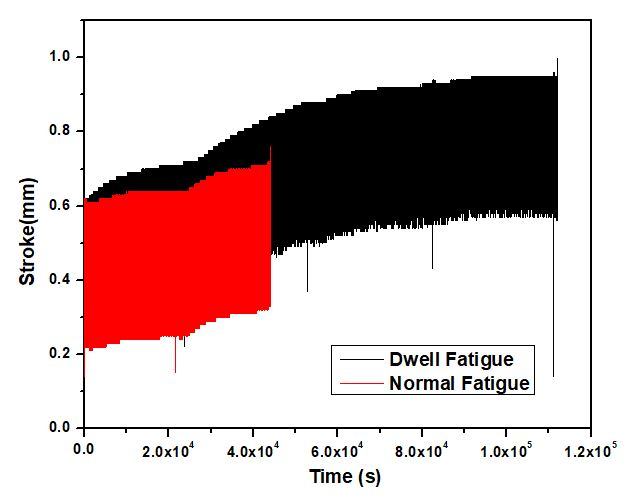
\includegraphics[width=\textwidth]{images/Dwell and cyclic.JPG}
        \caption{Cyclic Fatigue}
    \end{subfigure}
    \\
    \begin{subfigure}{0.60\textwidth}
        \includegraphics[width=0.70\textwidth]{\FatigueTest{S-N_Curve.eps}}
        \caption{S-N Curve for Ti-6242}
    \end{subfigure}    
\end{figure}

\end{frame}
%%%%%%%%%%%%%%%%%%%%%%% Thank You %%%%%%%%%%%%%%%%%%%%%%%%%%%

\begin{frame}[standout]
  Thank You
\end{frame}

%%%%%%%%% DSC Curve for Ti-6242
\begin{frame}{Measuring Beta Transus for Ti-6242}
\begin{figure}[H]
    \centering
    \begin{subfigure}{0.48\textwidth}
        \includegraphics[width=\textwidth]{\HeatTreatment{Ti6242-Heat-Graph.eps}}
        \caption{Heating Cycle}
        \label{fig:Ti-6242 Threshold}
    \end{subfigure}
    ~
    \begin{subfigure}{0.48\textwidth}
        \includegraphics[width=\textwidth]{\HeatTreatment{Ti6242-Cool-Graph.eps}}
        \caption{Cooling Cycle}
        \label{fig:Ti-6242 HT700}
    \end{subfigure}    
   
    \caption{DSC Curve for Ti-6242 @10 Kpm}
  
\end{figure}
\end{frame}

\end{document}
